%%==================================================
%% chapter04.tex for BIT Master Thesis
%% modified by yang yating
%% version: 0.1
%% last update: Dec 25th, 2016

%% modified by Meng Chao
%% version: 0.2
%% last update: May 29th, 2017
%%==================================================
\chapter{实验与结果}
\label{chap:EXPERIMENT}
We evaluate the LSD algorithm reliable performance on indoor and outdoor environment, recording with a hand-hold monocular camera. The trajectory is show in the mapping.

% 4.1
\section{Indoor Environment}
We evaluate the LSD algorithm hand holding camera in indoor environment. We test two time for the different sample key frames. The result is show in Fig.4 The picture (a) and (b) are the reference image and the key frame. The (c) and (d) are the reconstruction 3D map of the LSD-SLAM. The result is expressed the more key frames can be get the more detail of the environment, now that the noisy of the environment will affect the performance of LSD.

\begin{figure}
    \centering
       %\begin{minipage}{5cm}
       	  \subfigure[]
       	  {
          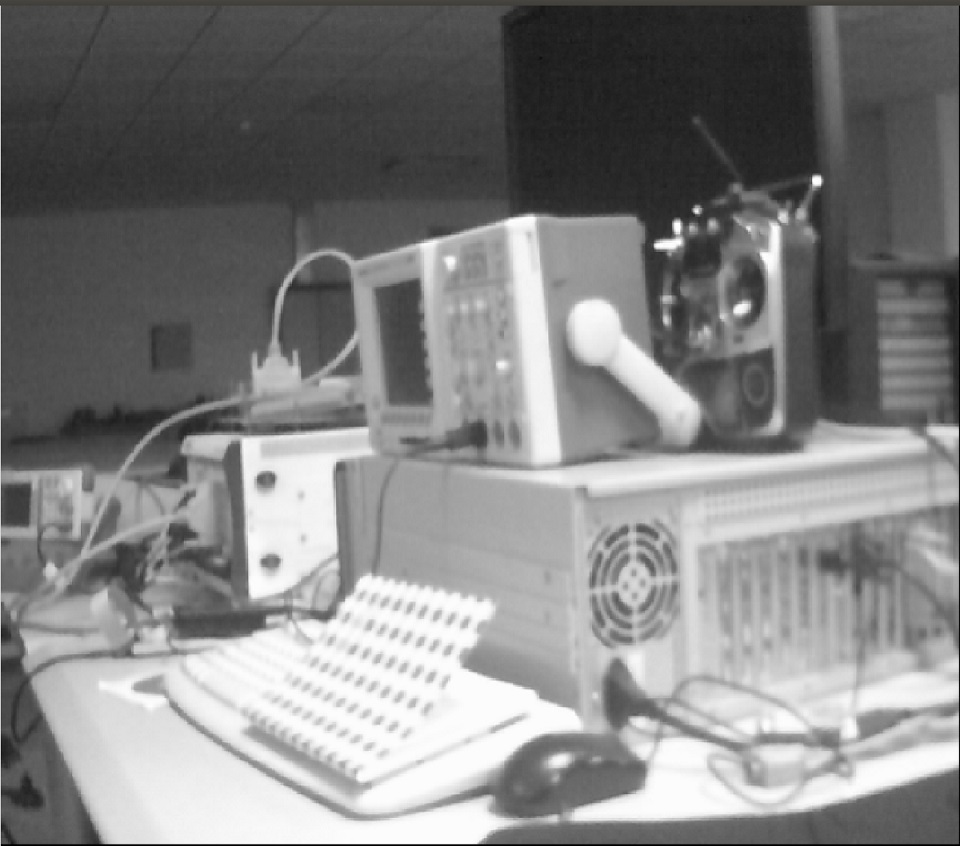
\includegraphics[scale=.2]{figures/Fig4(a)}          
          %\subcaption{}
          }                    
          \subfigure[]
       	  {
          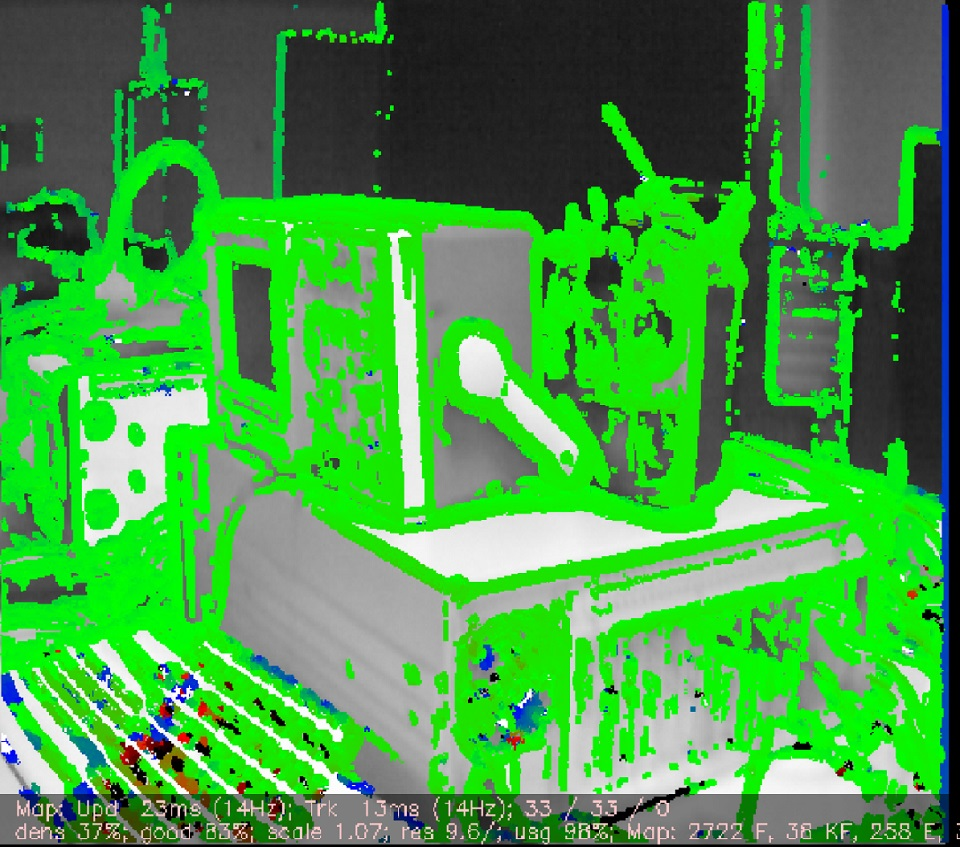
\includegraphics[scale=.2]{figures/Fig4(b)}
          %\subcaption{}
          }
          \hspace{0in}
     
          \subfigure[]
       	  {
          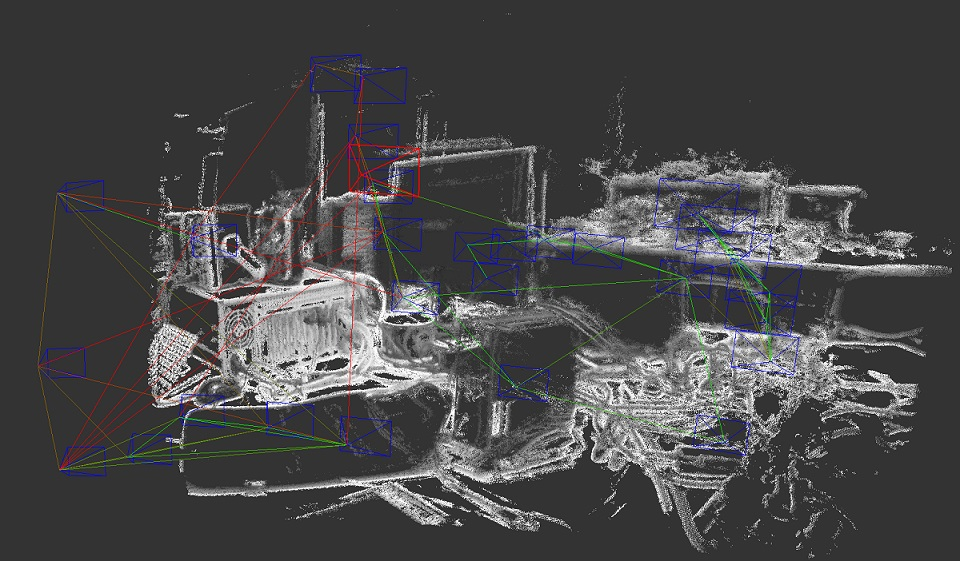
\includegraphics[scale=.25]{figures/Fig4(c)}
          %\subcaption{}
		  }
		  \subfigure[]
       	  {          
          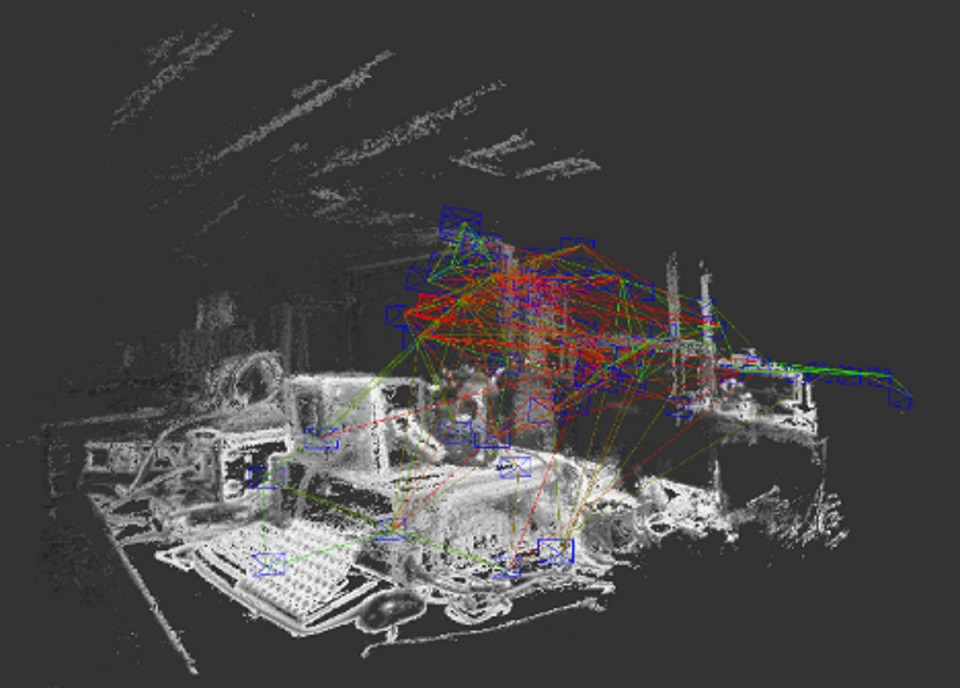
\includegraphics[scale=.2]{figures/Fig4(d)}
          %\subcaption{}
          }
          \hspace{0in}
       %\end{minipage}
     \caption{The indoor LSD-SLAM Map}
\end{figure}


\section{Outdoor Environment}
We evaluate the LSD-SLAM performance in outdoor. We accomplish the reconstruction the 3D map in diverse scene which is different distance. The result is expressed in Fig.5

The picture (a) and (b) are the different distance scene reference image for hand holding camera. The (c) and (d) is the reconstruction map of the LSD-SLAM. We can find that the mapping is completely reconstructed the scene information and the noisy is low in outdoor environment. This can be used in unmanned aerial vehicle(UAV) navigation and localization. The LSD-SLAM is reliable and robustness.

\begin{figure}
    \centering
       %\begin{minipage}{5cm}
       	  \subfigure[]
       	  {
          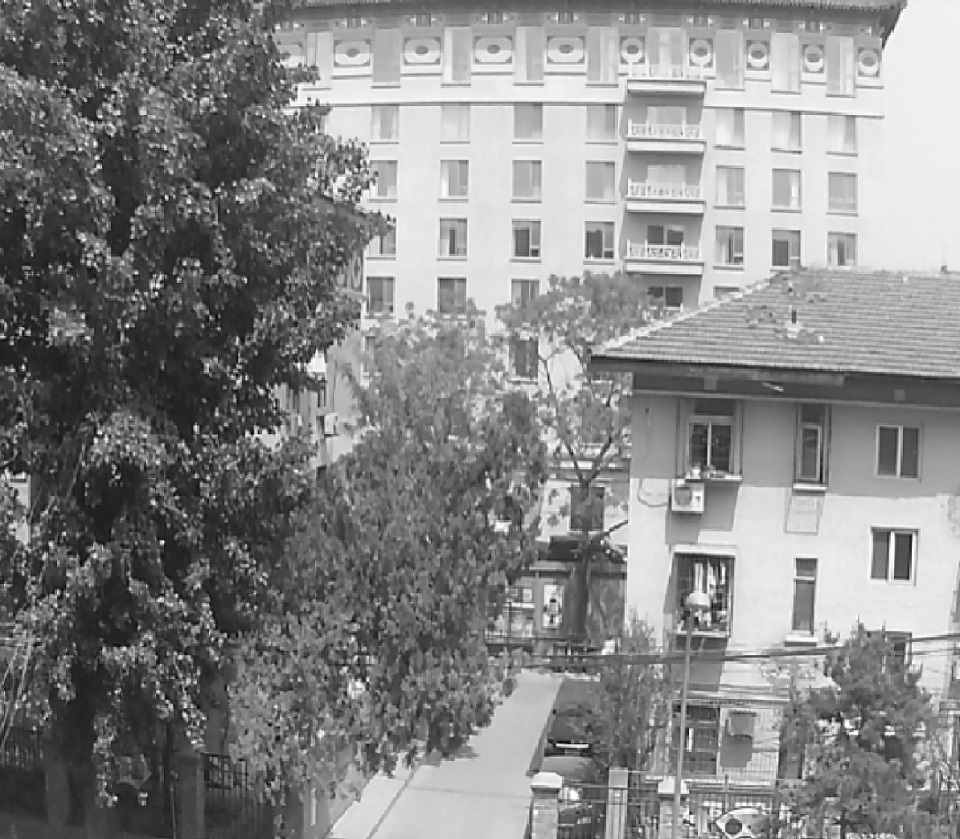
\includegraphics[scale=.2]{figures/Fig5(a)}          
          %\subcaption{}
          }                    
          \subfigure[]
       	  {
          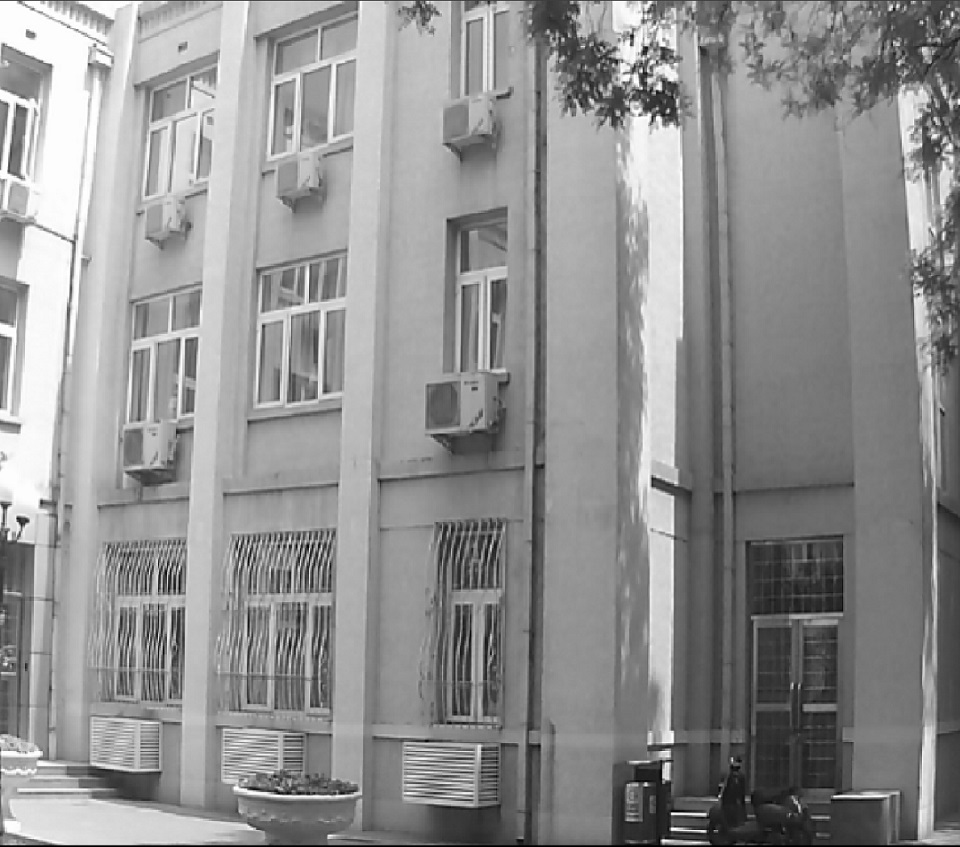
\includegraphics[scale=.2]{figures/Fig5(b)}
          %\subcaption{}
          }
          \hspace{0in}
     
          \subfigure[]
       	  {
          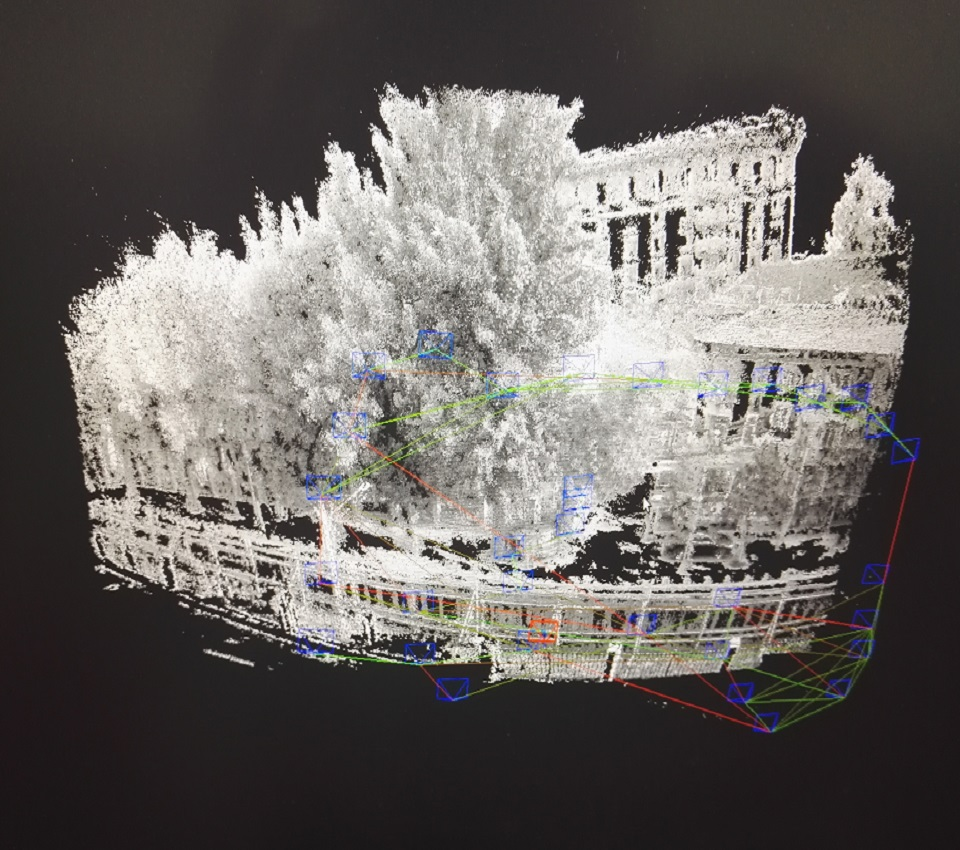
\includegraphics[scale=.25]{figures/Fig5(c)}
          %\subcaption{}
		  }
		  \subfigure[]
       	  {          
          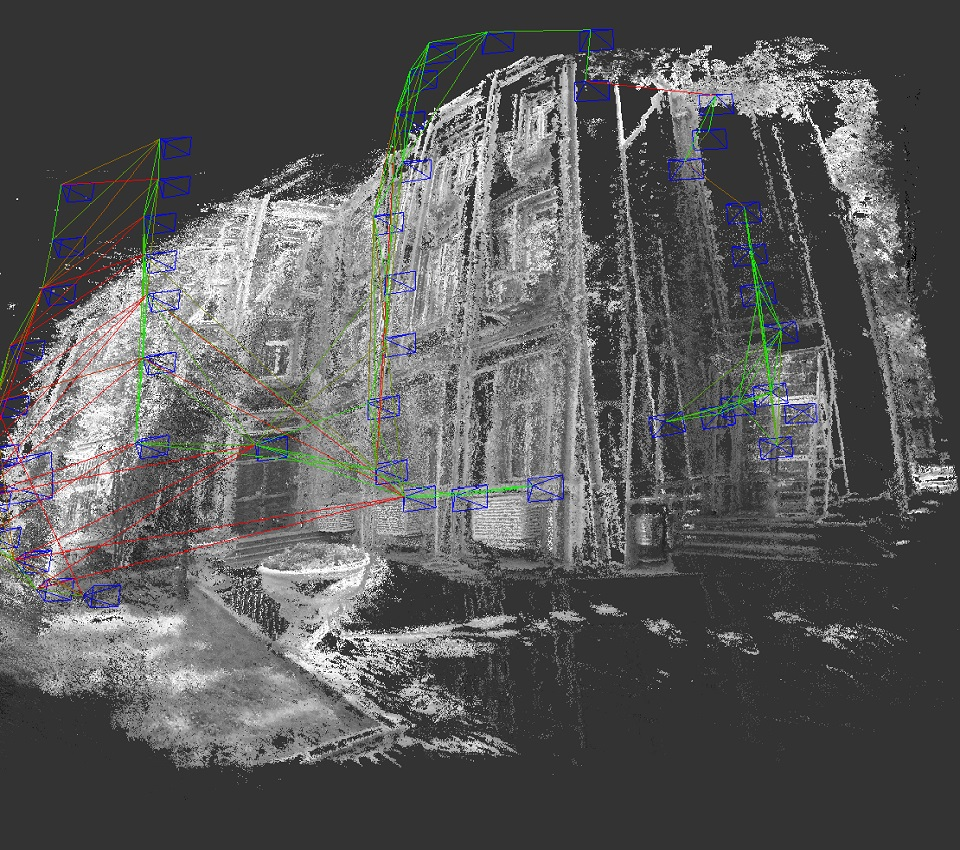
\includegraphics[scale=.2]{figures/Fig5(d)}
          %\subcaption{}
          }
          \hspace{0in}
       %\end{minipage}
     \caption{The outdoor LSD-SLAM Map}
\end{figure}

\section{Tum RGB-D Benchmark}

\begin{table}
\newcommand{\tabincell}[2]{\begin{tabular}{@{}#1@{}}#2\end{tabular}}
\centering

    \caption{Localization Error in Tum Dataset}     % NOTE!  caption goes _before_ the table contents !!
    \label{tab:font-sizes}
	\renewcommand\arraystretch{1.5}
    \begin{small}
    \begin{tabular}{p{2cm}p{1.5cm}p{1.5cm}p{1.5cm}}
    \hline

    \multicolumn{1}{c}{\multirow{3}{*}{Seq.}}
    & \multicolumn{3} {c} {\bfseries\tabincell{c} {Absolute Key Frame \\ Trajectory RMSE(cm)}} \\
    \cline{2-4}
    \multicolumn{1}{c}{}&   \multicolumn{1}{c}{\bfseries \tabincell{c}{LSD-SLAM} }      &     \multicolumn{1}{c}{\bfseries \tabincell{c}{ semi-dense \\mono-VO}}   & \multicolumn{1}{c}{\bfseries \tabincell{c}{ RGB-D \\SLAM}} \\	

    \cline{1-4}


  \multicolumn{1}{c}{fr2/desk}     &\multicolumn{1}{c}{5.65}      &\multicolumn{1}{c}{13.50}       &\multicolumn{1}{c}{2.58}   \\

  \multicolumn{1}{c}{Fr2/xyz}       &\multicolumn{1}{c}{2.15}      &\multicolumn{1}{c}{3.79}        &\multicolumn{1}{c}{1.34}   \\

  \multicolumn{1}{c}{sim/slowmo}    &\multicolumn{1}{c}{0.37}      &\multicolumn{1}{c}{2.21}        &\multicolumn{1}{c}{0.13}   \\

  \hline

    \end{tabular}
    \end{small}
\end{table}

The LSD-SLAM is evaluated on the Tum dataset. It is very challenging because of containing fast rotational movement, strong motion blur and rolling shutter artifacts. The result is displayed in tableⅠand compared with other algorithm for the localization accuracy.We use the very first depth map to bootstrap the system and get the correct initial scale.



